\documentclass{IEEEcsmag}

\usepackage[colorlinks,urlcolor=blue,linkcolor=blue,citecolor=blue]{hyperref}
\expandafter\def\expandafter\UrlBreaks\expandafter{\UrlBreaks\do\/\do\*\do\-\do\~\do\'\do\"\do\-}
\usepackage{upmath,color}


\jvol{XX}
\jnum{XX}
\paper{8}
\jmonth{Month}
\jname{Publication Name}
\jtitle{Publication Title}
\pubyear{2025}

\newtheorem{theorem}{Theorem}
\newtheorem{lemma}{Lemma}


\setcounter{secnumdepth}{0}
\usepackage[T1]{fontenc}
\usepackage{graphicx}
\usepackage{hyperref} 
\input{sec/preamble}
\input{sec/notations}

\begin{document}

\sptitle{Article Type: Regular}

\title{SpindleNet: Open-set Chinese Historical Text Recognition via Implicit Enhanced Component Representation}

\author{Xinming Zhang, Chang Liu, Yulong Bai, Yuqi Cui, Shu Tian}
\affil{University of Science and Technology Beijing, Beijing, 100084, China}

\markboth{THEME/FEATURE/DEPARTMENT}{THEME/FEATURE/DEPARTMENT}

\begin{abstract}
Open-set text recognition in Chinese historical texts remains challenging because of a vast array of ancient characters and a pronounced long-tail distribution, which leaves minimal samples for many rare tail classes. Mitigating this imbalance crucially helps recognize novel characters often hidden within these underrepresented categories. Moreover, Chinese characters share structural parts, making localized feature enhancement highly beneficial for both head and tail classes alike. We therefore propose SpindleNet, which bolsters local component representation by embedding a Radical Residual Module and expanding the channel capacity of middle layers to capture fine-grained details. To constrain parameter growth and complexity, we shorten the depth of subsequent layers, resulting in a distinctive "spindle" shape. Extensive evaluations on three difficult Chinese ancient book datasets, TKH, MTH1000, and MTH1200, show that SpindleNet significantly surpasses existing methods, offering improved feature extraction for tail-class characters and thereby establishing a new state-of-the-art performance across varied tasks.
\end{abstract}

\maketitle

\input{sec/0_exp_info}
\section{Introduction}
\input{figures/database_long_tail.tex}
China, with its extensive and culturally rich history, has accumulated a vast array of historical documents spanning centuries of scholarship, governance, and literary expression. These documents offer incomparable academic and artistic value, presenting essential insights into linguistics, cultural anthropology, and social development. Consequently, there has been an upsurge of research interest directed towards the analysis and recognition of historical documents~\cite{jinic21,hde,obc306}. As researchers delve deeper into this field, new methodologies have been developed to contend with the inherent complexities that arise from the condition and content of such documents.

Historical texts often pose challenges distinct from modern text recognition, largely due to the presence of severe physical degradation. Stains, tears, and ink bleeding result from the natural aging process or prolonged exposure to environmental factors. These forms of damage cause substantial visual distortions in the character glyphs, making accurate recognition difficult even for advanced methods~\cite{Hong2021, Dou2021}. Additionally, scribal variations, regional styles, and calligraphic differences across dynasties create a remarkable diversity in character shapes. This complexity further necessitates specialized modeling strategies that account for inconsistent ink intensities and complex stroke structures, which are seldom seen in modern documents. This uniqueness of historical documents also emphasizes the importance of domain knowledge and domain-specific model architectures that can robustly handle the variety of possible degradations.

Aside from the visual difficulties introduced by document quality, another key issue in historical document recognition originates from the distribution of the data itself, where certain characters are extremely frequent while others scarcely appear~\cite{obcmk2}. This long-tailed character occurrence distribution presents a formidable obstacle, as it forces models to overfit high-frequency characters while largely ignoring the underrepresented, albeit significant, tail characters. Although the long-tailed distribution also affects other text recognition tasks~\cite{fudanvi}, historical document recognition manifests a substantially higher degree of ``longtailness,'' measured by the Gini Coefficient~\cite{tailsurvey} (see Figure~\ref{fig:moretailed}). This metric highlights the pronounced skew in historical texts, wherein a small set of characters occupies the majority of instances. Consequently, designing methods that can accommodate these skewed distributions is crucial for achieving reliable recognition performance.

Moreover, new characters in test data tend to be situated at the distribution's tail~\cite{jinic21}, effectively combining open-set recognition with long-tail challenges. The emergence of these previously unseen characters, often archaic or region-specific, can significantly degrade the performance of models trained solely on common categories. In such scenarios, robust generalization to novel classes is not merely beneficial but essential, as the inability to correctly identify or interpret new characters could jeopardize critical historical interpretations. Recent research efforts have thus begun to investigate strategies that explicitly encode prior knowledge or structural information to mitigate the negative effects of sparse tail samples~\cite{Tang2022}.

To address this confluence of obstacles, existing methods exploit the radical information of each character, capitalizing on the fact that radicals often act as semantic or phonetic building blocks~\cite{denseran}. Since individual radicals may appear across both head and tail classes, the utilization of radical information has shown promising generalization capabilities for recognizing previously unseen characters~\cite{fewran,zhang20pr}. By breaking down unfamiliar glyphs into known components, radical-based methods can approximate the correct representation of characters appearing in the tail. On the other hand, Zhang et al.~\cite{sanicdar23} proved that leveraging component information significantly enhances tail class performance by effectively sharing knowledge between more common and extremely rare characters. Despite the effectiveness of these techniques, a significant limitation arises from their reliance on radical-level annotations, which require laborious expert labeling for each character’s constituent parts. As a result, annotation costs balloon in large-scale projects, and difficulties arise in transferring such methods to different scripts or new sets of characters.

In this work, we propose a strategy that aims to circumvent the requirement for labor-intensive radical annotations by adopting a visual matching approach~\cite{vsdf}. Our goal is to continue exploiting the similarity among character components while implicitly emphasizing detailed feature modeling. Specifically, we develop a novel spindle backbone network that allocates an increased number of parameters to the layers responsible for capturing component-level features, a design choice motivated by the desire to amplify the network’s sensitivity to the subtleties of shared parts across characters. Inspired by insights from mobile neural network architectures~\cite{mobile} and investigations into feature dissection~\cite{dissection}, the spindle backbone focuses on expanding the capacity of middle layers (conv2 and conv3), which are crucial for extracting mid-level texture-like features. We argue that these middle layers are inherently better at representing the strokes and partial forms characteristic of radicals or sub-character components. By contrast, high-frequency signals in shallow layers are often detrimental to generalization~\cite{hfharm,hffilter}, so our design refrains from widening the shallowest layers. 

In parallel, the deeper layers of the network are streamlined to sustain a compact overall parameter footprint, thus preserving both high inference speed and reduced VRAM usage. This balanced approach ensures that the network remains deployable in resource-constrained environments such as digital libraries and cultural heritage archives that maintain large-scale digitization workflows. Combining these elements, the spindle backbone emerges as a design that strategically prioritizes mid-level features without significantly inflating computational cost.

Summarizing these motivations, we present a spindle network with narrow shallow layers and narrow deep layers but wider middle layers, enabling stronger learning of stroke-like structures that can be reused across head, tail, and even novel classes. In addition, the Radical Residual Module (RSM) is incorporated to further boost the representational power of the features corresponding to character radicals. By integrating both spatial and channel attention while drawing upon prior knowledge of 265 common radical templates, the RSM can guide the network to focus on relevant spatial regions more effectively. This enhanced spatial attention ultimately contributes to improved discrimination of fine-grained radical or stroke patterns, thus elevating recognition performance for both seen and unseen classes.

The RSM integrates spatial attention mechanisms that attend to local character regions where radicals are likely to be found, and it uses channel attention to calibrate the importance of different feature maps. These processes benefit from the partial supervision derived from the radical templates, which provide gentle guidance in highlighting areas of interest. In doing so, the network is naturally steered to emphasize consistent component features that are characteristic of radicals across an extensive range of text samples. As a result, the representation of novel characters is bolstered, and the tail classes witness improvements in recognition accuracy that are especially vital in historical document contexts where annotated data is scarce or unevenly distributed.

We conducted architectural ablation studies to verify that the spindle design outperforms both the traditional pyramid design and the reverse pyramid design in terms of overall accuracy and robustness. Experimental outcomes reveal that our emphasis on mid-level feature expansion aligns with the structural complexities of historical documents, allowing better generalization to atypical or damaged characters. This observed superiority underscores the practical value of carefully tailoring the network architecture to address the multiple demands of historical text recognition, where visual degradation, long-tail distributions, and open-set challenges frequently coexist~\cite{Bai2023}.

As a structural-knowledge-free approach, the proposed method also exhibits compelling recognition abilities when confronted with novel classes, significantly reducing the labor involved in adapting the model to newly uncovered historical materials or freshly excavated scripts. Empirically, our network's capacity to handle both head and tail classes sees consistent gains in experiments, reinforcing its applicability in large-scale digitization efforts that require not just sheer accuracy, but also the flexibility to accommodate continuous discoveries of rare and unknown characters. Ultimately, by sidestepping expensive radical-level annotations while still capturing compositional character information, the proposed approach marks a step forward in making historical text recognition more scalable, comprehensive, and adept at handling the myriad challenges ingrained in ancient manuscripts.

In summary, the main contributions of this paper can be considered as follows:
\begin{itemize}
\item we introduce the Radical Residual Module (RSM), which strategically exploits the intrinsic similarity among character radicals to enhance recognition performance, especially for novel or infrequently appearing characters. By incorporating both spatial and channel attention mechanisms, the RSM guides the model to focus on shared substructures that transcend individual glyphs, thereby improving the system’s capacity to generalize beyond the training set. 
\item Building upon this radical-aware framework, we then propose a spindle network designed to deepen the extraction of character components. This architecture widens the intermediate layers where sub-character features and texture-like patterns are most salient, leveraging commonalities across various components and improving the representation of complex or degraded characters. The enhanced capacity in mid-level layers amplifies the model’s ability to capture nuanced details, leading to tangible gains in recognizing unseen or rare glyphs and thus addressing the challenges posed by long-tailed distributions. 
\item we validate the effectiveness and versatility of our method through extensive experiments on three challenging Chinese ancient book datasets, namely TKH, MTH1000, and MTH1200. Empirical results clearly demonstrate that our approach achieves state-of-the-art performance in this domain, underscoring its practicality for large-scale historical document digitization. By integrating radical-informed cues with a balanced architectural design, our framework not only achieves higher accuracy but also exhibits robust generalization across both abundant and rare character classes.
\end{itemize}


\begin{figure*}[t]
    \begin{center}
    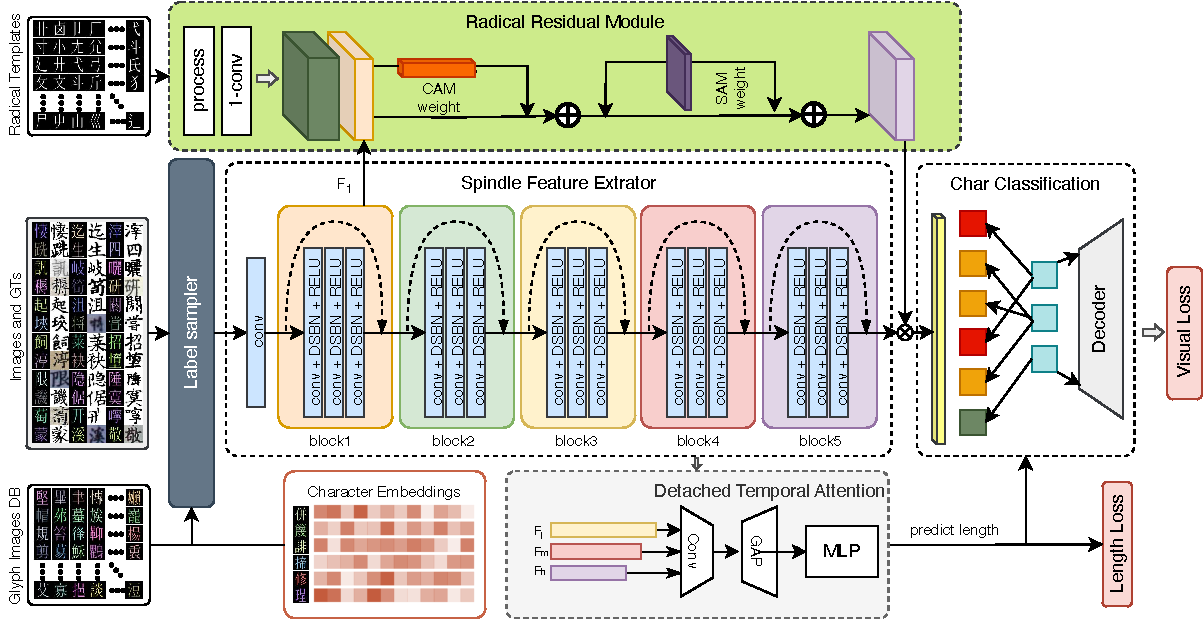
\includegraphics[width=1.0\linewidth]{figures/overall.pdf}
    \end{center}
    \caption{Overview. This framework is composed of four modules: a feature extraction module, a character length module, a decoder module, and a Radical Residual Module.}
    \label{fig:overall}
\end{figure*}

\section{Related Works}
\label{sec:related_works}

In this section, we provide a comprehensive review of prior studies in layout analysis, text recognition, and the long-tailed distribution problem, with a particular emphasis on their relevance to historical text recognition tasks. Various approaches, including both classical optical character recognition (OCR) systems and more recent deep learning-based techniques, have been explored to address the unique challenges posed by historical documents~\cite{liu2019survey, bishop2006pattern}. Nevertheless, the intricacies involved in digitizing centuries-old texts, which often include noise, uneven ink spread, and archaic writing styles, have propelled researchers to devise specialized strategies. This section outlines the challenges inherent in current methods and sets the stage for our proposed solution, while emphasizing that effective historical text recognition necessitates a careful consideration of layout complexities, language-specific characteristics, and the long-tailed distribution of characters~\cite{jla}.

\subsection{Historical Text Recognition}

Document digitization plays an essential role in preserving cultural heritage by converting physical documents into digital formats, enabling efficient storage, retrieval, and analysis. The transformation of historical texts into machine-readable data has been significantly facilitated by OCR technologies, which range from traditional rule-based methods to advanced deep neural networks~\cite{conway2010, yadav2021handwritten}. Among its key components, text recognition has garnered significant attention as it is central to transforming digitized documents into formats that allow historians, linguists, and archivists to conduct comprehensive research~\cite{jla}.

Historical text recognition methods are generally categorized into two main approaches: character-based methods and sequence-based methods. Both offer unique strengths but also face challenges when applied to historical documents, including the presence of rare symbols, blurred ink traces, and nonlinear text flow~\cite{chetarly22}. These difficulties underscore the need for robust and adaptable approaches that can handle the variations introduced by time and usage.

\subsubsection{Character-Based Methods}

Character-based methods focus on processing individual characters by decomposing the recognition pipeline into locating characters, recognizing them, and grouping them into meaningful text lines~\cite{papytwin}. This strategy has been widely studied due to its ability to explicitly model character-level details, which can be advantageous when dealing with highly complex or irregular character shapes. However, it remains particularly challenging in historical contexts because the documents often exhibit degraded quality with broken or smudged characters caused by age-related wear and imperfect printing processes~\cite{broken}. Historical materials may also include handwritten texts with widely varying writing styles, introducing a layer of complexity as the differences in stroke density and curvature can hinder recognition accuracy~\cite{obc306}. Furthermore, the frequency of characters is often heavily skewed, implying that a few commonly used characters dominate the distribution while a vast number of rare characters rarely appear~\cite{fewran}. These rare characters may include novel symbols or archaic ligatures~\cite{hde,ligarature} that never appear in standard training datasets, thus complicating the development of universal or language-agnostic models. Despite these difficulties, the character-based approach remains a foundational method because its modularity allows for fine-grained control over each step of the recognition pipeline and provides a mechanism to explicitly address rare or newly discovered characters during the digitization of historically significant texts.

\subsubsection{Sequence-Based Methods}

Sequence-based methods aim to recognize entire lines of text directly from images, bypassing the need for explicit character segmentation~\cite{eccvfork,jinic21}. In these methods, a network is typically trained with line-level annotations, which are easier to obtain in large quantities compared to the detailed labeling required for character-level training~\cite{adams2019sequence}. Although sequence-based methods have reduced annotation burdens and demonstrated remarkable performance in modern OCR tasks, they still face limitations. First, they struggle to handle rare characters efficiently because imbalanced datasets often overemphasize the few high-frequency symbols while neglecting many low-frequency ones. Second, they exhibit sensitivity to variations in text layout and structure, which is especially problematic in historical documents with intricate page designs or non-standard formatting. Third, their reliance on implicit representations makes it difficult to generalize to unseen characters or to explicitly model novel symbols, thereby limiting their usefulness when encountering entirely new character shapes. While sequence-based methods are appealing for large-scale digitization efforts that seek to rapidly process line-level data, tasks that require detailed character-level analysis can suffer from the reduced interpretability and adaptability of these models. In this work, we adopt a character-oriented perspective to address the unique challenges of historical text recognition because it allows more direct handling of long-tailed and novel character distributions.

\subsection{The Long-Tailed Distribution Problem}

The long-tailed distribution problem is a pervasive issue in machine learning, particularly in tasks where a few classes dominate the dataset (referred to as head classes), while a majority of classes are underrepresented (referred to as tail classes)~\cite{tailsurvey}. This imbalance has far-reaching implications for model training, making it difficult to achieve high accuracy for underrepresented classes. Standard optimization methods often overfit to the head classes, capturing only limited nuances from rare classes. In text recognition, this skewed distribution leads to misclassification of rare characters, an issue that is magnified in historical text corpora where unique or archaic symbols appear infrequently~\cite{garcia2018improved}.

\subsubsection{Existing Solutions}

Existing solutions to the long-tailed problem can be situated within three primary strategies that seek to balance the representation of head and tail classes, thereby improving the overall performance of recognition systems. Data-side approaches focus on balancing the data distribution by introducing class-balancing sampling, which allocates more training emphasis on underrepresented characters~\cite{upsam}, or by adopting data augmentation techniques, such as generating synthetic samples to bolster the diversity of tail classes~\cite{cutmix, smote, hzsl}. Other strategies involve optimization-side approaches, where loss reweighting schemes allocate higher importance to rare classes~\cite{focal,otem} and additional regularization terms guide the model toward learning more generalizable features~\cite{fudanvi,sanicdar23,logvar}. Finally, model-side approaches concentrate on architectural modifications, including ensemble methods that aggregate predictions from multiple specialized models~\cite{fle,flmoe}, and classifier adaptations that adjust decision boundaries to address imbalanced distributions~\cite{normrob}. Each line of research offers distinct advantages, but combining these perspectives often leads to more robust solutions. Indeed, recent progress suggests that hybrid approaches that integrate data augmentation with reweighted loss functions or specialized network modules can achieve state-of-the-art results for long-tailed recognition tasks~\cite{chen20dgan}.

\subsubsection{Zero-Shot Learning and Its Relevance}

Zero-shot learning presents an extreme case of the long-tailed problem, where certain classes in the test set are absent from the training phase entirely~\cite{gzsl-survey,olt}. By leveraging shared attributes between head and tail classes, zero-shot methods enable models to generalize to unseen categories without direct sample supervision~\cite{shen22}. This capability is particularly valuable in historical text recognition contexts, where new or archaic characters may suddenly appear in a document. When used judiciously, zero-shot learning frameworks reduce the reliance on meticulously annotated data, and they can exploit the compositional nature of characters, such as the shared radicals or strokes in handwritten scripts. Despite the promise of these techniques, they also require careful architectural design to ensure the accurate transfer of learned knowledge to genuinely new symbols.

\subsection{Long Tails in Historical Text Recognition}

Historical text recognition presents unique challenges in addressing long-tailed distributions. The frequency distribution of characters in historical corpora often reflects natural language use, where common characters dominate the text while rare symbols occur sporadically~\cite{yang2022survey}. This phenomenon is exacerbated by the limited availability of annotated historical datasets, which not only restricts the variety of character exemplars but also intensifies the scarcity of training samples for tail classes. Researchers have attempted to alleviate these difficulties by exploiting shared knowledge between head and tail classes, such as radical composition~\cite{obcmk2,sanicdar23,fudanvi} or stroke-based features that capture fundamental structural elements of characters~\cite{taktak}. Although these approaches demonstrate improvements, they typically rely on detailed annotations that demand expert knowledge and are not easily transferable across different scripts or languages.

To overcome these limitations, we propose a novel approach that implicitly leverages the shared components of characters within a carefully designed backbone network. By emphasizing part-level features during feature extraction, our method reduces reliance on explicit annotations while enhancing performance for tail classes and novel characters. In particular, by focusing on the compositional structure of characters rather than their overall shape, we improve the model's ability to generalize to unusual or unseen symbols that often arise in historical documents. This approach addresses the core challenges of historical text recognition in a more general and scalable manner, offering a pathway to digitize vast collections of historical texts that exhibit highly imbalanced and evolving character distributions.

%-------------------------------
% Additional References in BibTeX Format
%-------------------------------
% Please insert the following references into your .bib file or reference list as needed.

\input{sec/3_method_v1_cat}
\input{sec/4_experiments_v1_cat}
\section{Conclusion}

In this paper, we have demonstrated that the intrinsic similarity among character components can be leveraged to substantially enhance recognition performance for characters situated in the tail of long-tail distributions. This improvement is especially critical for new or infrequently encountered characters, as their representation is often underemphasized in traditional deep learning models. By recognizing and exploiting these shared structural elements, the network gains an enriched understanding of how individual strokes or radical components form complete characters, ultimately boosting accuracy where it is most needed.

Moreover, we introduced the spindle-shaped network architecture as a powerful means of extracting and refining local character component features. This design strategically expands channel capacity in mid-level layers, facilitating a richer embedding space and promoting more reliable feature representations that capture subtle distinctions between visually similar glyphs. The resultant focus on local components not only bolsters recognition of the rarest characters but also provides a more robust framework for accommodating newly encountered symbols. Through additional analyses, we verified the effectiveness of SpindleNet in adapting to both head and tail classes, ensuring balanced performance across the entire character set.

Extensive experiments conducted on three challenging Chinese ancient book datasets, namely TKH, MTH1000, and MTH1200, further validate the advantages of our method. The outcomes confirm that SpindleNet achieves state-of-the-art performance, surpassing conventional solutions by handling extreme data imbalance and preserving fidelity for high-frequency characters. In challenging historical textual corpora that feature a broad and often sparsely sampled set of characters, such improved recognition capabilities are indispensable for accurate transcription and subsequent scholarly research.

Looking ahead, we plan to extend our framework to a weakly-supervised training paradigm, a direction that has already shown promise in scene text recognition tasks. This approach could reduce the burden of precise annotations while potentially increasing the volume of available training samples. By integrating weak labels or partial annotations, future models may become even more adept at unraveling the intricate forms of rare and unseen characters, thereby advancing the state of the art for ancient document understanding.


\bibliographystyle{splncs04}
\bibliography{ref/a,ref/refs,ref/all.bib}

\end{document}

